\documentclass[8pt]{beamer}

\usepackage[utf8]{inputenc}
\usepackage{default}
\usepackage{hyperref}
\usepackage{textpos}
\usepackage{verbatimbox}
\usetheme{Copenhagen}

\title{Deep Learning}
\subtitle{WaveNet: From article to TensorFlow code}
\author{Tero Keski-Valkama}
\institute{
\includegraphics[height=1.4cm]{CybercomG_logo_Classic_RGB.png}}
\date{2010-01-19}

\addtobeamertemplate{frametitle}{}{%
\begin{textblock*}{100mm}(10.95cm,-0.8cm)

\includegraphics[height=0.8cm]{cybercom-blue.png}
\end{textblock*}}


\begin{document}

\frame{\titlepage}
 
\begin{frame}
\frametitle{What is WaveNet}

\begin{itemize}
 \item WaveNet: A Generative Model for Raw Audio by Aaron van den Oord et al. @ DeepMind: https://arxiv.org/pdf/1609.03499.pdf
 \item WaveNet Tensorflow implementation by Igor Babuschkin et al: https://github.com/ibab/tensorflow-wavenet
\end{itemize}

\end{frame}

\begin{frame}[fragile]
\frametitle{Causal layer}
\begin{columns}
\begin{column}{0.5\textwidth}
 
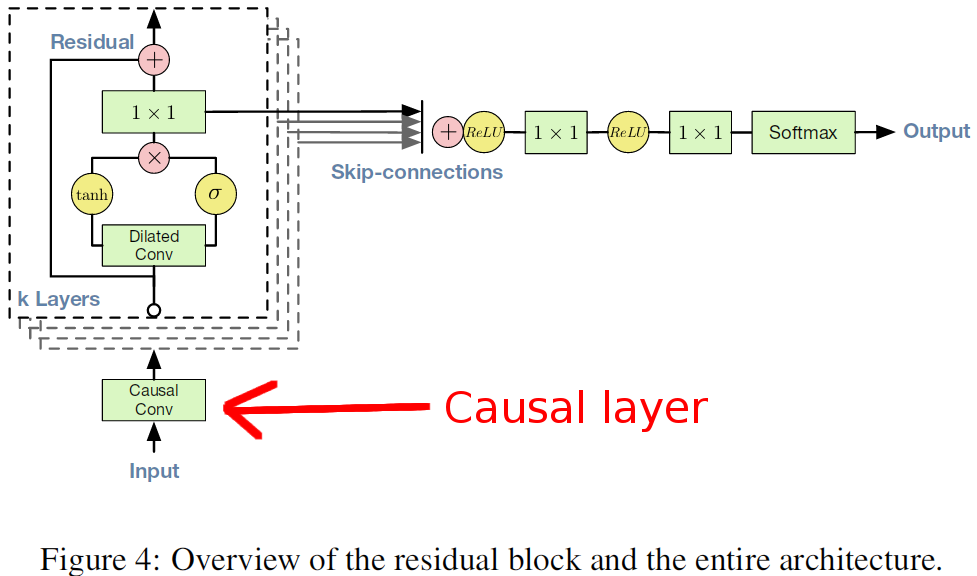
\includegraphics[width=0.9\textwidth]{./dl3_images/causal_layer.png}

\end{column}
\begin{column}{0.5\textwidth}
 
 \textcolor{blue}{wavenet/model.py\#L172}
 
 \begin{verbnobox}[\tiny]
def _create_causal_layer(self, input_batch):
    '''Creates a single causal convolution layer.
    The layer can change the number of channels.
    '''
    with tf.name_scope('causal_layer'):
        weights_filter = self.variables['causal_layer']['filter']
    return causal_conv(input_batch, weights_filter, 1)
 \end{verbnobox}
\end{column}
\end{columns} 
 
\end{frame}

\begin{frame}[fragile]
\frametitle{Causal convolution}
\begin{columns}
\begin{column}{0.5\textwidth}
 
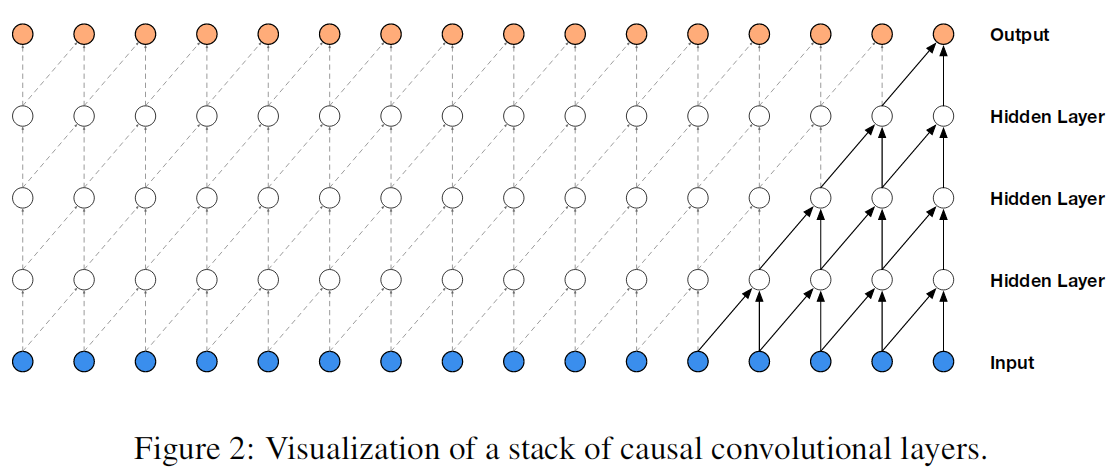
\includegraphics[width=0.9\textwidth]{./dl3_images/causal_convolutions.png}

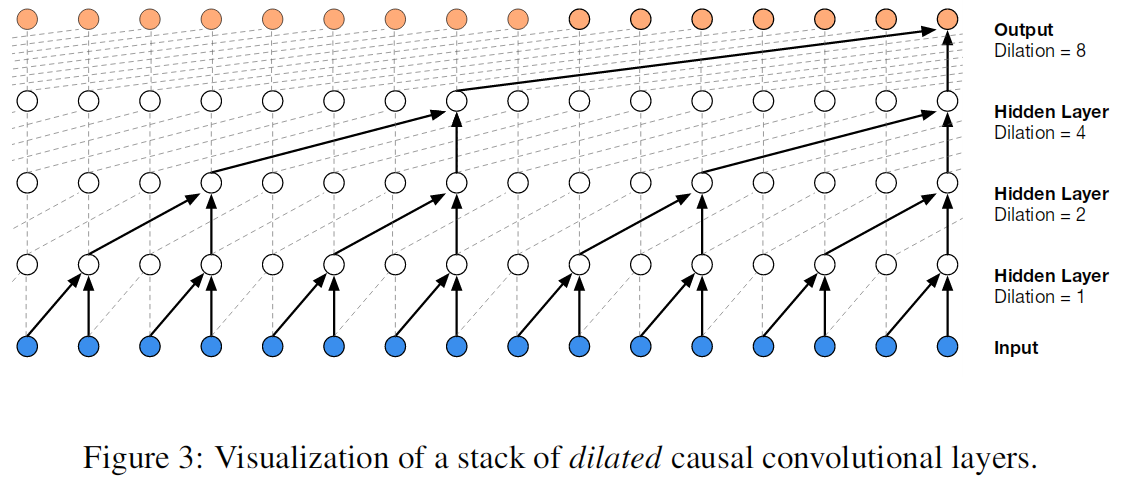
\includegraphics[width=0.9\textwidth]{./dl3_images/dilated_causal_convolutions.png}

\end{column}
\begin{column}{0.5\textwidth}
 
 \textcolor{blue}{wavenet/ops.py\#L27}
 
 \begin{verbnobox}[\tiny]
def time_to_batch(value, dilation, name=None):
    with tf.name_scope('time_to_batch'):
        shape = tf.shape(value)
        pad_elements = dilation - 1 - (shape[1] + dilation - 1) % dilation
        padded = tf.pad(value, [[0, 0], [0, pad_elements], [0, 0]])
        reshaped = tf.reshape(padded, [-1, dilation, shape[2]])
        transposed = tf.transpose(reshaped, perm=[1, 0, 2])
        return tf.reshape(transposed, [shape[0] * dilation, -1, shape[2]])

def batch_to_time(value, dilation, name=None):
    with tf.name_scope('batch_to_time'):
        shape = tf.shape(value)
        prepared = tf.reshape(value, [dilation, -1, shape[2]])
        transposed = tf.transpose(prepared, perm=[1, 0, 2])
        return tf.reshape(transposed,
                          [tf.div(shape[0], dilation), -1, shape[2]])

def causal_conv(value, filter_, dilation, name='causal_conv'):
    with tf.name_scope(name):
        # Pad beforehand to preserve causality.
        filter_width = tf.shape(filter_)[0]
        padding = [[0, 0], [(filter_width - 1) * dilation, 0], [0, 0]]
        padded = tf.pad(value, padding)
        if dilation > 1:
            transformed = time_to_batch(padded, dilation)
            conv = tf.nn.conv1d(transformed, filter_, stride=1, padding='SAME')
            restored = batch_to_time(conv, dilation)
        else:
            restored = tf.nn.conv1d(padded, filter_, stride=1, padding='SAME')
        # Remove excess elements at the end.
        result = tf.slice(restored,
                          [0, 0, 0],
                          [-1, tf.shape(value)[1], -1])
    return result
 \end{verbnobox}
\end{column}
\end{columns} 
 
\end{frame}

\begin{frame}[fragile]
\frametitle{Stack of convolutional layers}
\begin{columns}
\begin{column}{0.5\textwidth}
 
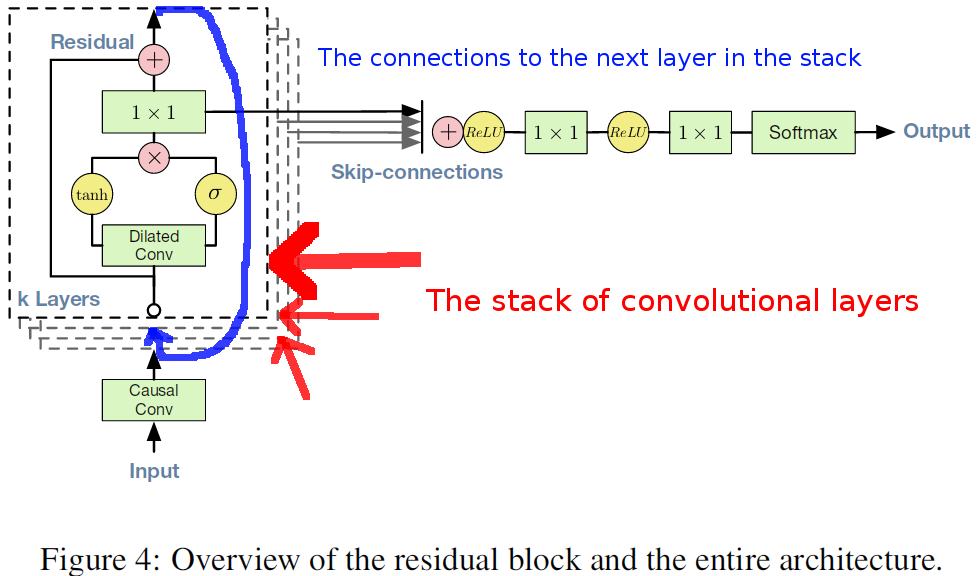
\includegraphics[width=0.9\textwidth]{./dl3_images/stack_of_convolutional_layers.png}

\end{column}
\begin{column}{0.5\textwidth}
 
 \textcolor{blue}{wavenet/model.py\#L300}
 
 \begin{verbnobox}[\tiny]
  # Add all defined dilation layers.
  with tf.name_scope('dilated_stack'):
      for layer_index, dilation in enumerate(self.dilations):
          with tf.name_scope('layer{}'.format(layer_index)):
              output, current_layer = self._create_dilation_layer(
                  current_layer, layer_index, dilation)
              outputs.append(output)
 \end{verbnobox}
\end{column}
\end{columns} 
 
\end{frame}

\begin{frame}[fragile]
\frametitle{Convolutional dilation layer}
\begin{columns}
\begin{column}{0.5\textwidth}
 
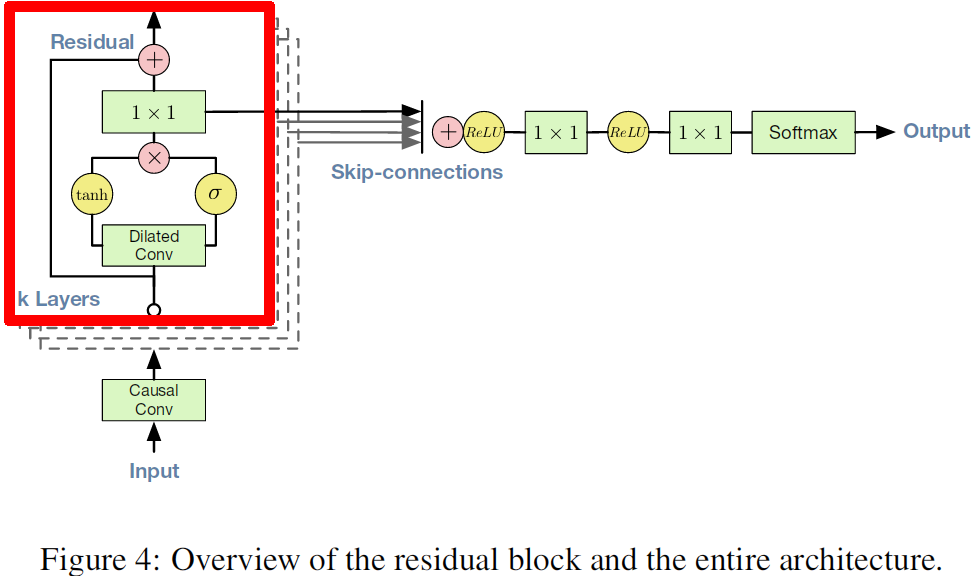
\includegraphics[width=0.9\textwidth]{./dl3_images/dilation_layer.png}

\end{column}
\begin{column}{0.5\textwidth}
 \textcolor{blue}{wavenet/model.py\#L181}
 
 \begin{verbnobox}[\tiny]
def _create_dilation_layer(self, input_batch, layer_index, dilation):
        '''Creates a single causal dilated convolution layer.
        The layer contains a gated filter that connects to dense output
        and to a skip connection:
               |-> [gate]   -|        |-> 1x1 conv -> skip output
               |             |-> (*) -|
        input -|-> [filter] -|        |-> 1x1 conv -|
               |                                    |-> (+) -> dense output
               |------------------------------------|
        Where `[gate]` and `[filter]` are causal convolutions with a
        non-linear activation at the output.
        '''
        variables = self.variables['dilated_stack'][layer_index]

        weights_filter = variables['filter']
        weights_gate = variables['gate']

        conv_filter = causal_conv(input_batch, weights_filter, dilation)
        conv_gate = causal_conv(input_batch, weights_gate, dilation)

        ... CODE FOR OPTIONAL BIASES ...

        out = tf.tanh(conv_filter) * tf.sigmoid(conv_gate)

        # The 1x1 conv to produce the residual output
        weights_dense = variables['dense']
        transformed = tf.nn.conv1d(
            out, weights_dense, stride=1, padding="SAME", name="dense")

        # The 1x1 conv to produce the skip output
        weights_skip = variables['skip']
        skip_contribution = tf.nn.conv1d(
            out, weights_skip, stride=1, padding="SAME", name="skip")

        ... CODE FOR OPTIONAL BIASES / HISTOGRAM OUTPUT ...
        
        return skip_contribution, input_batch + transformed
 \end{verbnobox}

\end{column}
\end{columns} 
 
\end{frame}

\begin{frame}[fragile]
\frametitle{1X1 Convolutions (dilation layer)}
\begin{columns}
\begin{column}{0.5\textwidth}
 
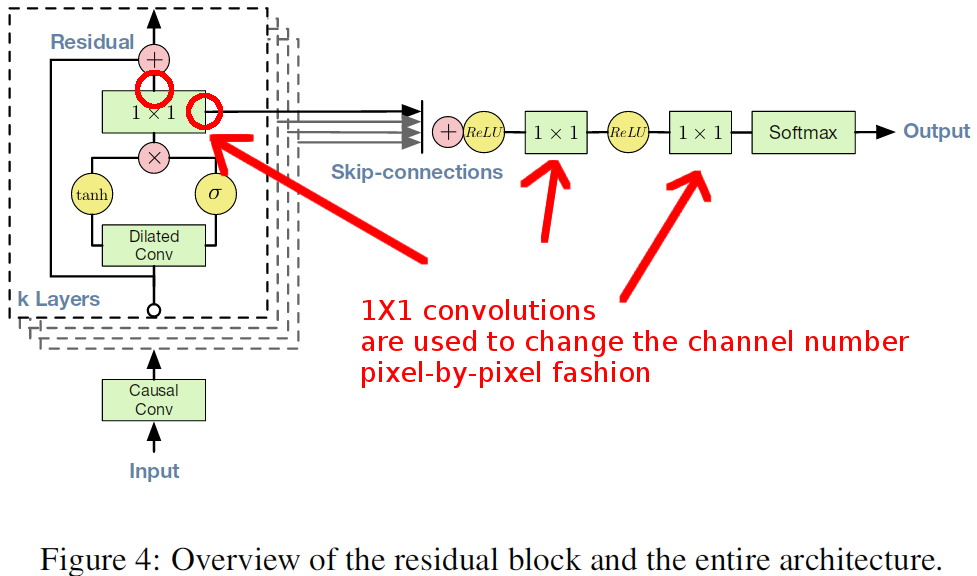
\includegraphics[width=0.9\textwidth]{./dl3_images/1x1_convolutions.png}

\end{column}
\begin{column}{0.5\textwidth}
 
\textcolor{blue}{wavenet/model.py\#L127}
 
\begin{verbnobox}[\tiny]
    current['dense'] = create_variable(
        'dense',
        [1,
            self.dilation_channels,
            self.residual_channels])
    current['skip'] = create_variable(
        'skip',
        [1,
            self.dilation_channels,
            self.skip_channels])
\end{verbnobox}

\textcolor{blue}{wavenet/model.py\#L212}
 
 \begin{verbnobox}[\tiny]
    # The 1x1 conv to produce the residual output
    weights_dense = variables['dense']
    transformed = tf.nn.conv1d(
        out, weights_dense, stride=1, padding="SAME", name="dense")

    # The 1x1 conv to produce the skip output
    weights_skip = variables['skip']
    skip_contribution = tf.nn.conv1d(
        out, weights_skip, stride=1, padding="SAME", name="skip")
\end{verbnobox}

\end{column}
\end{columns} 
 
\end{frame}

\begin{frame}[fragile]
\frametitle{1X1 Convolutions (postprocessing)}
\begin{columns}
\begin{column}{0.5\textwidth}
 
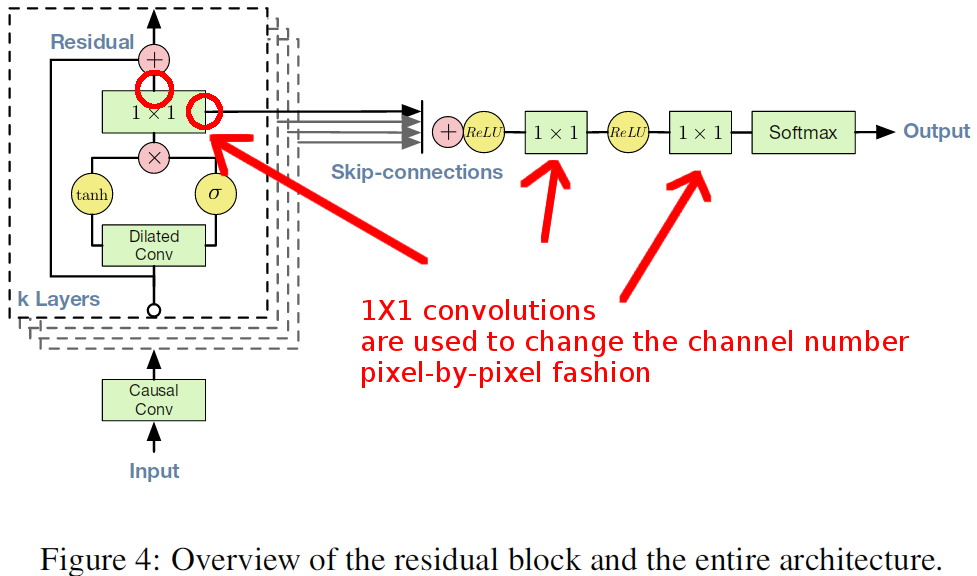
\includegraphics[width=0.9\textwidth]{./dl3_images/1x1_convolutions.png}

\end{column}
\begin{column}{0.5\textwidth}
 
 \textcolor{blue}{wavenet/model.py\#L155}
 
\begin{verbnobox}[\tiny]
    current['postprocess1'] = create_variable(
        'postprocess1',
        [1, self.skip_channels, self.skip_channels])
    current['postprocess2'] = create_variable(
        'postprocess2',
        [1, self.skip_channels, self.quantization_channels])
\end{verbnobox}

 \textcolor{blue}{wavenet/model.py\#L324}
 
 \begin{verbnobox}[\tiny]
    w1 = self.variables['postprocessing']['postprocess1']
    w2 = self.variables['postprocessing']['postprocess2']
    ... CODE FOR OPTIONAL BIASES / HISTOGRAM OUTPUT ...
    # We skip connections from the outputs of each layer, adding them
    # all up here.
    total = sum(outputs)
    transformed1 = tf.nn.relu(total)
    conv1 = tf.nn.conv1d(transformed1, w1, stride=1, padding="SAME")
        ... CODE FOR OPTIONAL BIASES ...
    transformed2 = tf.nn.relu(conv1)
    conv2 = tf.nn.conv1d(transformed2, w2, stride=1, padding="SAME")
\end{verbnobox}

\end{column}
\end{columns} 
 
\end{frame}

\end{document}

